
\chapter{Αλγόριθμοι μείωσης διαστάσεων}
\numberwithin{equation}{section}

\section{Γραμμική μείωση διαστάσεων}
\par
Όλες οι τεχνικές μείωσης διαστάσεων στις οποίες έχουμε αναφερθεί μέχρι στιγμής είναι κατεξοχήν τεχνικές μείωσης της διάστασης του χώρου των χαρακτηριστικών. Μάλιστα το ιδιαίτερο χαρακτηριστικό τους είναι ότι αποτελούν μεθόδους οι οποίες σέβονται την γραμμικότητα. Η μέθοδος \textlatin{PCA} για παράδειγμα η οποία αποτελεί μια απο τις γνωστότερες αλλά και πιο ισχυρές μεθόδους γραμμικής μείωσης διαστάσεων λειτουργεί καλά αν τα σημεία των δεδομένων είναι κατανεμημένα σε ένα υπερεπίπεδο. Επίσης, όπως αναλύθηκε στην ενότητα (2.2) η μέθοδος \textlatin{PCA} προβάλλει στις διευθύνσεις μέγιστης διασποράς. Τέλος όπως εξηγήσαμε στο προηγούμενο κεφάλαιο η ανάλυση ιδιοτιμών-ιδιοδιανυσμάτων του μητρώου συσχέτισης αποκαλύπτει την διάσταση του υπερεπιπέδου στο οποίο τα δεδομένα είναι διεσπαρμένα. 
\par
Με άλλα λόγια δηλαδή η διάσταση είναι ένα μέτρο του πλήθους των ελεύθερων μεταβλητών που είναι "υπεύθυνες" για τον τρόπο με τον οποίο μεταβάλλεται ένα σήμα, δηλαδή για την πραγματική πληροφορία την οποία κωδικοποιούν τα δεδομένα. 
\par
Παρότι ο αλγόριθμος \textlatin{PCA} αποτελεί μία πολύ ισχυρή και ευρέως χρησιμοποιούμενη μέθοδο μείωσης της διάστασης υπάρχουν περιπτώσεις στις οποίες η μέθοδος αποτυγχάνει. Τέτοιες είναι περιπτώσεις κατα τις οποίες ο μηχανισμός παραγωγής των δεδομένων είναι έντονα μη γραμμικός με αποτέλεσμα τα δεδομένα να κείτονται σε πιο περίπλοκες πολλαπλότητες. Ας πάρουμε για παράδειγμα τις εξισώσεις \\
\begin{center}
$x_{1}=r cos\theta, \quad x_{2}=rsin\theta$
\end{center}
Προφανώς απο τις παραπάνω εξισώσεις είναι φανερό ότι το $x$ βρίσκεται στην περιφέρεια κύκλου ακτίνας $r$. Πρόκειται δηλαδή για πρόβλημα μονοδιάστατης πολλαπλότητας αφού αρκεί μια μόνο μεταβλητή για την περιγραφή των δεδομένων. Η παράμετρος αυτή είναι η απόσταση κατα μήκος της περιφέρειας απο ένα σημείο(αφετηρία) πάνω στην περίμετρο του κύκλου. Αν λοιπόν εφαρμόσουμε την μέθοδο \textlatin{PCA} στο παραπάνω σύνολο δεδομένων τότε η απάντηση που θα μας δώσει για την διάσταση των δεδομένων θα είναι, λανθασμένα προφανώς, ίση με δύο. 
\par
Περιπτώσεις όπως οι παραπάνω απαιτούν αλγορίθμους μείωσης διάστασης και εξαγωγής χαρακτηριστικών οι οποίοι να λαμβάνουν υπόψιν την γεωμετρία του προβλήματος ώστε να μπορούν να εξάγουν αποτελεσματικά συμπεράσματα για την διάσταση των δεδομένων. Στον τομέα της υπολογιστικής όρασης για παράδειγμα, ο οποίος όπως αναφέραμε και παραπάνω αποτελεί βασικό κομμάτι της εν λόγω διατριβής, απαιτούνται κατεξοχήν αλγόριθμοι μη γραμμικής μείωσης διαστάσεων αφού οι εικόνες ή τα χαρακτιριστκά των εικόνων τα οποία αποτελούν τα δεδομένα μας είναι κατα κύριο λόγο μη γραμμικά. 

\section{Μη γραμμική μείωση διαστάσεων}
\par
Υπάρχει λοιπόν μια ευρεία γκάμα εφαρμογών οι οποίες απαιτούν αλγορίθμους μη γραμμικής μείωσης διαστάσεων. Αυτό συμβαίνει διότι στις συγκεκριμένες εφαρμογές η γεωμετρική αναπαράσταση των δεδομένων είναι τέτοια ώστε απαιτείται να βρεθεί μια ενσωμμάτωση μικρότερης διάστασης η οποία βρίσκεται "κρυμμένη" στον χώρο των αρχικών διαστάσεων. Θα πρέπει μάλιστα κατά την διαδικασία αυτή να ληφθούν προφανώς υπόψιν τα γεωμετρικά χαρακτηριστικά του χώρου των δεδομένων. 
\par
Έχει πολύ μεγάλη σημασία στο σημείο αυτό να κατανοήσουμε τι εννοούμε όταν αναφερόμαστε στα γεωματρικά χαρακτηριστικά του προβλήματος. Το πιο χαρακτηριστικό και ευρέως χρησιμοποιούμενο παράδειγμα για τον σκοπό αυτό είναι ένα τεχνητό σετ δεδομένων, με την όνομασία \textlatin{Swiss Roll} το οποίο φαίνεται στην παρακάτω εικόνα. \\
\vspace{1.0cm}
\begin{figure}[h]
\centering
%\hspace*{2.5cm}
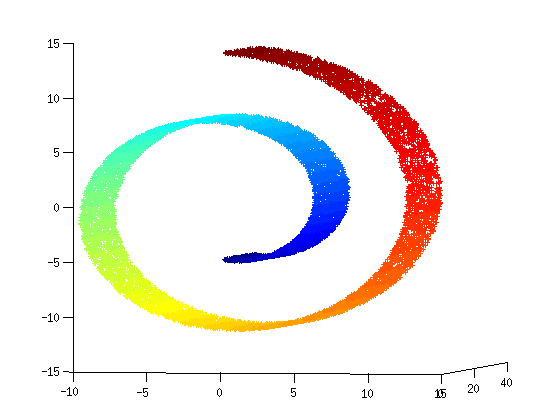
\includegraphics[scale=0.8]{figs/2.png}
\newline
\caption{ \textlatin{Swiss Roll Synthetic Dataset}.} 
\end{figure}
\vspace{1.0cm}
\par
Αυτό που αξίζει να παρατηρηθεί λοιπόν στο παραπάνω σετ δεδομένων είναι ότι αν για παράδειγμα διαλέξουμε κάποιο οποιοδήποτε σημείο του απο την κόκκινη περιοχή και προσπαθήσουμε να βρούμε ποιά δεδομένα αποτελούν κοντινότερους γείτονες του σημείου αυτού πιθανότατα θα πέφταμε στην παγίδα, όπως και οι τεχνικές γραμμικής μείωσης διαστάσεων, να πούμε ότι κάποια σημεία απο την μπλέ περιοχή βρίσκονται και αυτά στην γειτονιά του σημείου που διαλέξαμε. Αυτό προφανώς είναι λάθος αφού απο τον χρωματισμό των παραπάνω δεδομένων αντιλαμβανόμαστε ότι στην πραγματικότητα τα μπλέ δεδομένα βρίσκονται πολύ μακριά απο τα κόκκινα. Ο παραπάνω εσφαλμένος συλλογισμός αναπαρίσταται στο παρακάτω γράφημα.
\par
\begin{figure}[h!]
\centering
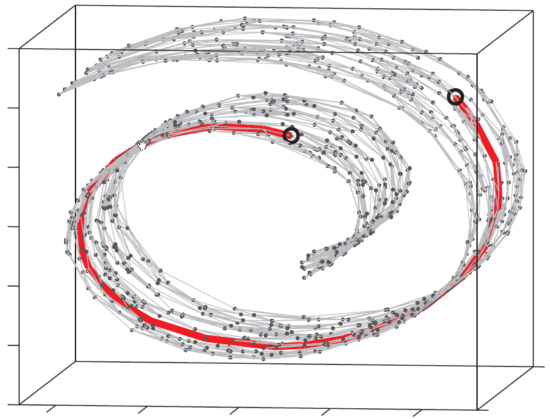
\includegraphics[scale=0.5]{figs/3.png}
\newline
\caption{\textlatin{Swiss Roll Synthetic Dataset Manifold Learning Path.}} 
\end{figure}
\par
\vspace*{1cm}
Αντιλαμβανόμαστε λοιπόν, μέσω της παραπάνω απεικόνισης ότι θα πρέπει να ληφθεί υπόψιν η γεωμετρία του προβλήματος ώστε σε καμιά περίπτωση υπολογίζοντας κοντινότερες αποστάσεις να συμπεριλάβουμε το αρχικό και το τελικό σημείο ως κοντινούς γείτονες, ενώντάς τα απευθείας μεταξύ τους. Αυτή είναι και η διαφορά των αλγορίθμων μη γραμμικής μείωσης διαστάσεων με αυτούς της γραμμικής. Για να γίνει πλήρως κατανοητός ο τρόπος μείωσης των διαστάσεων του παραπάνω σετ δεδομένων, δίνεται η απεικόνιση των δεδομένων σε χώρο χαμηλής διάστασης μετά απο την εφαρμογή αλγορίθμου μη γραμμικής μείωσης διαστάσεων.
\clearpage
\begin{figure}[t]
\centering
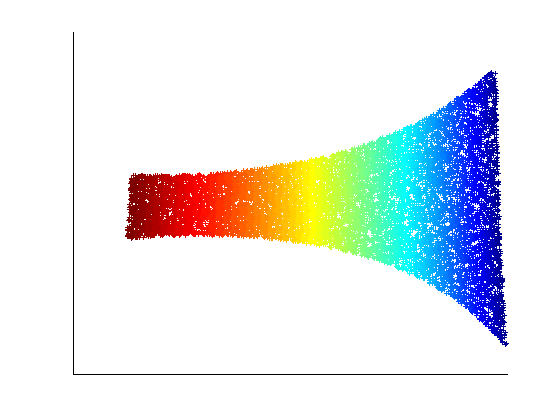
\includegraphics[scale=0.8]{figs/4.png}
\newline
\caption{\textlatin{Dimensionality Reduction with LLE - 3D (K=16,d=2).}} 
\end{figure}
\par
\vspace*{1cm}
Απο την παραπάνω απεικόνιση μπορούμε να φανταστούμε ότι κάνοντας μείωση των διαστάσεων στην πραγματικότητα "ξετυλίξαμε" το \textlatin{Swiss Roll} και έτσι απο τον αρχικό χώρο των τριών διαστάσεων στην πραγματικότητα η εγγενής διάσταση των δεδομένων είναι ίση με δύο. Στις επόμενες ανότητες θα γίνει παρουσίαση των πιο γνωστών μεθόδων μη γραμμικής μείωσης διαστάσεων καθώς επίσης θα γίνει και η μαθηματική τους ανάλυση.


\subsection{\textlatin{ISOMAP}}
\par
Ένας βασικός αλγόριθμος μη γραμμικής μείωσης διαστάσεων είναι ο αλγόριθμος Ισομετρική απεικόνιση \textlatin{(Isometric Mapping - ISOMAP)}. Ο αλγόριθμος αυτός υιοθετεί την άποψη ότι μόνο οι γεωδαιτικές αποστάσεις μεταξύ όλων των ζευγών των σημείων των δεδομένων μπορούν να αντικατοπτρίσουν την πραγματική δομή της πολλαπλότητας του προβλήματος. Η παραπάνω διατύπωση αντικατοπτρίζει το παράδειγμα που δόθηκε στο γράφημα (3.2), και τονίζει το γεγονός ότι οι Ευκλείδιες αποστάσεις μεταξύ σημείων μιας πολλαπλότητας δεν μπορούν να την αναπαραστήσουν ικανοποιητικά διότι σημεία (στο γράφημα τα δύο σημεία που έχουν επισυμανθεί με μαύρους κύκλους) που είναι απομακρυσμένα μεταξύ τους, σύμφωνα με την γεωδαιτική απόσταση, μπορεί να θεωρηθούν, λανθασμένα, κοντικά ως προς την Ευκλείδια απόστασή τους.
\par
Ουσιαστικά η μέθοδος \textlatin{ISOMAP} είναι μια παραλλαγή του αλγορίθμου \textlatin{Multi Dimensional Scaling - MDS}, με την διαφορά ότι οι Ευκλείδιες αποστάσεις αντικαθίστανται απο τις αντίστοιχες γεωδαιτικές κατά μήκος της πολλαπλότητας των δεδομένων. Η ουσία του αλγορίθμου είναι να εκτιμηθούν σωστά οι γεωδαιτικές αποστάσεις μεταξύ σημείων τα οποία είναι απομακρυσμένα μεταξύ τους. Ο αλγόριθμος μπορεί να χωριστεί σε δύο βασικά βήματα:
\par
Βήμα-1: \\ Για κάθε σημείο $x_{i},i=1,1\ldots,n$, υπολόγισε τους πλησιέστερους γείτονες και κατασκέυασε έναν γράφο $G(V,E)$ του οποίου οι κορυφές αναπαριστούν πρότυπα εισόδου και οι ακμές συνδέουν τους πλησιέστερους γείτονες. Οι παράμετροι $k$ ή $\epsilon$ είναι παράμετροι που καθορίζονται απο τον χρήστη). Στις ακμές ανατίθενται βάρη σύμφωνα με τις αντίστοιχες Ευκλείδιες αποστάσεις (για τους πλησιέστερους γείτονες αυτή είναι μια καλή προσέγγιση της γεωδαιτικής απόστασης).
\par
Βήμα-2: \\ Υπολόγισε ανα ζεύγος την γεωδαιτική απόσταση για όλα τα ζεύγη κατα μήκος των συντομότερων διαδρομών μέσα στον γράφο. Το πιο σημαντικό σημείο, είναι ότι η γεωδαιτική απόσταση μεταξύ δύο οποιονδήποτε σημείων της πολλαπλότητας μπορεί να προσεγγιστεί μέσω της συντομότερης διαδρομής που ενώνε τα δύο σημείο στο γράφο $G(V,E)$. Ο πιο γνωστός αλγόριθμος υλοποίησης της παραπάνω διαδικασίας είναι ο αλγόριθμος \textlatin{Djikstar} με πολυπλοκότητα $\mathcal{O}(n^{2}\ln n + n^{2}k)$, μέγεθος απαγορευτικό για τις περισσότερες πρακτικές εφαρμογές.
\par
Εφόσον έχουν εκτελεστεί τα δύο αυτά βήματα είμαστε πλέον σε θέση νε εφαρμόσουμε την κλασική μέθοδο \textlatin{MDS}. Το πρόβλημα λοιπόν απο εδώ και στο εξής γίνεται ισοδύναμο με την εφαρμογή της ανάλυσης ιδιοδιανυσμάτων του αντίστοιχου μητρώου \textlatin{Gram} και την επιλογή των \textlatin{m} περισσότερο σημαντικών ιδιοδιανυσμάτων για την αναπαράσταση του χώρου χαμηλής διάστασης. Μετά απο αυτή την αναπαράσταση, οι Ευκλείδιες αποστάσεις μεταξύ των σημείων του χώρου χαμηλής διάστασης ταιριάζουν με τις αντίστοιχες γεωδαιτικές αποστάσεις στην πολλαπλότητα του αρχικού χώρου υψηλής διάστασης. Όπως και στις μεθόδους \textlatin{PCA} και \textlatin{MDS} η διάσταση \textlatin{m} εκτιμάται απο το πλήθος των \textlatin{m} περισσότερο σημαντικών ιδιοτιμών. Αποδεικνύεται τέλος ότι η μέθοδος \textlatin{ISOMAP} ασυμπτωτικά ($n \rightarrow \inf$) θα ανακτήσει την αληθινή διάσταση για ένα σύνολο δεδομένων μη γραμμικής πολλαπλότητας.

\subsection{\textlatin{Laplassian Eigenmaps}}
\par


\subsection{\textlatin{LLE}}
\par

